\section{Dead Reckoning}\label{section:theory-dead-reckoning}
%Dead-Reckoning \citep{thesis:dead-reckoning}, as previously described in \secref{section:dead-reckoning}, is a movement tracking technique. In the previous section the concept was described, whereas in this section it will be described thoroughly in regards to the mathematical details.
%
%%\subsection{Pedestrian Dead Reckoning}
This section is based on theory from \citep{misc:PedestrianDeadReckoningSystem}.
The pedestrian DR uses the accelerometer and the gyroscope to detect steps and estimate the step-length.
Steps can be detected in 3 different ways, peak detection, zero crossing detection, and flat zone detection.

Peak detection finds the maxima and minima of the accelerometer output, and when a maximum is found it looks for the next minimum which determines a step, and vice versa. 
Every step has acceleration phase followed by a deceleration phase, peak detection finds these two phases by finding a local maximum and minimum that are close to each other, as seen in \figref{figure:peak-detection}.

Zero crossing detection checks where the accelerometer output crosses the x axis, with the heuristic that a step has a minimum and a maximum duration. 
As a step has three crossings of the x axis, first one is where it starts to accelerate, second is when the acceleration stops and the deceleration begins, and third is when the deceleration stops and the step is finished. 
These three crossings can be seen in \figref{figure:zero-crossing}.

Flat zone detection constrains the user to stop in between each step, and find the flat zones in the graph.
A flat zone is a zone on the graph where oscillation is not large enough to be included as a step.\fxnote{mangler nogle passende maalinger til den her som har pauser ind i mellem hvert skridt.}
\begin{figure}[H]
\centering
\includegraphics[trim=0 8cm 0cm 8cm, clip,scale=0.5]{media/peak-detection}
\caption{Peak detection finding one step.}
\label{figure:peak-detection}
\end{figure}

\begin{figure}[H]
\centering
\includegraphics[trim=0 8cm 0cm 8cm, clip,scale=0.5]{media/zero-crossing}
\caption{Zero crossing determining a step.}
\label{figure:zero-crossing}
\end{figure}

After finding the step, the step length can be determined by a linear combination of walking velocity and variance of the accelerometer, \eqref{eq:steplength}. \fxnote{er usikre på denne formel, vi mener v er noise fra accelerometer men er ikke sikker}
The walking distance, \eqref{eq:walkingdistance}, is the accumulated value of all the steps, which were found using the previously described algorithms and the step length equation.
\begin{equation}\label{eq:steplength}
	Step length = \alpha * f + \beta * v + \gamma \\
\end{equation}
\begin{equation}\label{eq:walkingdistance}
	Walking distance = \sum\limits_{i=1}^{n} (\alpha * f_i + \beta * v_i + \gamma)
\end{equation}
where,
\begin{itemize}
	\item[$\alpha , \beta$] is weights of walking parameters.
	\item[$\gamma$] is a constant.
	\item[$f_i$] is the walking velocity of the i-th step.
	\item[$v_i$] is the acceleration variance of the i-th step.
\end{itemize}

These formulas can be erroneous as the location of the phone can change which creates bad inputs in the calculation of the walking distance.
Determining the location of the phone is therefore important in pedestrian dead reckoning i.e if it is in the pocket, bag, or hand. But as this project is constraint to having the phone in a fixed position, phone location awareness as it is not necessary.

\section{Position Calculations}\label{sec:position-calculations}
In order to develop a game where a user moves to control the game, it is necessary to register these movements and calculate a position. 
Calculating positions can be done by analysing the data given from the accelerometer in the phone.
The output of the accelerometer is the accelerations of the three axis' of the accelerometer.
\figref{figure:acceleration-chart} and \figref{figure:velocity-chart} shows two graphs with each graph showing three steps.
\figref{figure:acceleration-chart} is the acceleration along the y-axis of the phone. 
\figref{figure:velocity-chart} is the velocity along the y-axis of the phone.
The velocity is calculated by taking the integral of the acceleration, the formula is as follows:
\begin{equation*}
v(T) = \int_0^T \! a(t) \, \mathrm{d}t
\end{equation*} 
where, $v(T)$ is the velocity at time $T$, and $a(t)$ is the acceleration at time $t$.

A graph with accelerations and a graph with the corresponding velocities can be seen in \figref{figure:acceleration-chart} and \figref{figure:velocity-chart}, respectively.

\begin{figure}[H]
	\centering	
	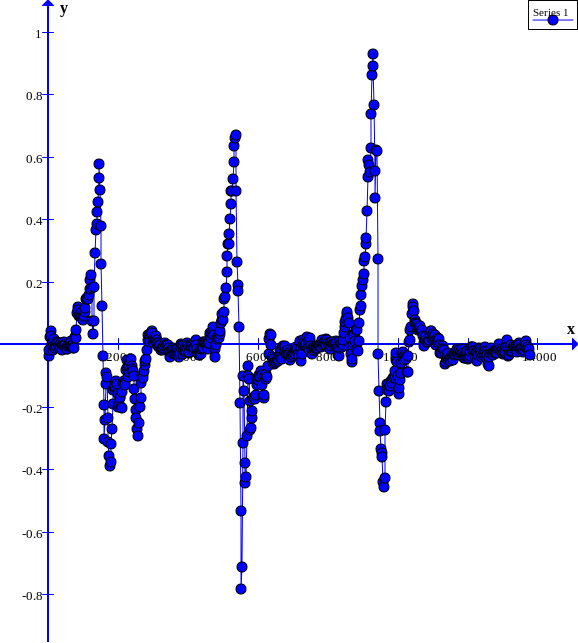
\includegraphics[scale=0.4, trim=0cm 2cm 0cm 2cm]{media/gnuplot/acceleration.pdf}
	\caption{Acceleration readings over three steps.}
	\label{figure:acceleration-chart}
\end{figure}

\begin{figure}[H]
	\centering	
	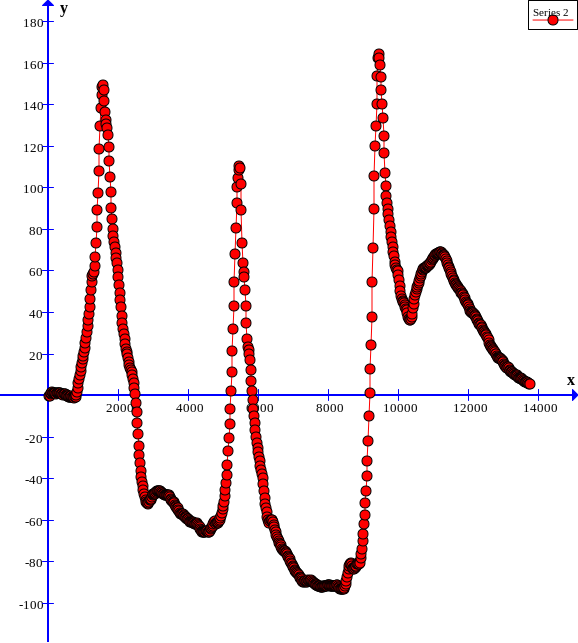
\includegraphics[scale=0.4, trim=0cm 2cm 0cm 2cm]{media/gnuplot/velocity.pdf}
	\caption{Velocity calculations over three steps.}
	\label{figure:velocity-chart}
\end{figure}

The velocity graph is smoother than the acceleration graph because each point on the velocity graph is a summation of the area of the acceleration graph.

To determine the position, the area under the velocity graph is calculated by taking the integral of the velocity over time, as seen in the following equation:

\begin{equation}\label{eq:integral-velocity}
     s(T) = \int_0^T v(t)\mathrm{d}t 
\end{equation}
where, $s(T)$ is the distance at time $T$, and $v(t)$ is the velocity at time $t$. 

The value can be used in conjunction with the previous position to calculate an approximation of the new position.
The actual values can be observed by video footages of people sidestepping with the phone.
As seen in the graphs, noise exists and should be corrected by use of filters.
%step detection
%step-length estimation
%Phone location awareness
%
%Calculate the double integration:
%accelerometer -> velocity -> step-length.

%teknikker til DR
%beregner skridt ud fra velocity.
%augument inertial/magnetic sensor (IMMU)
%Pedestrian 


%implementations teknikker
%http://www.diydrones.com/profiles/blogs/a-simple-deadreckoning
%http://www.gamasutra.com/view/feature/3230/dead_reckoning_latency_hiding_for_.php
%http://www.mmorpg.com/discussion2.cfm/post/2228522#2228522
%http://stackoverflow.com/questions/1261119/how-to-implement-dead-reckoning-when-turning-is-involved
%http://www.comp.lancs.ac.uk/~kristof/research/notes/deadreck/deadreck.html
%Direction

%Length

%Noise

%Extended Kalman Filter

%DRA-1